\begin{center}
    \section*{\fontsize{20}{20}\selectfont Chapter 4}
\end{center}
\vspace{10mm}

\section{Implementation and Result Analysis}
This chapter delves into the implementation specifics and the corresponding result analysis of the proposed EHealth platform. It details the technical environment in which the system was developed and deployed, the procedures applied for data preprocessing, and the step-by-step model implementation strategies. Furthermore, the chapter systematically presents the evaluation metrics used to measure system effectiveness, a detailed performance analysis utilizing the experimental results, and a structured discussion of the key findings. Finally, the system's performance is benchmarked against existing state-of-the-art approaches to highlight its practical improvements and contributions to telemedicine technology.

\subsection{Environment Setup}
The EHealth platform was implemented utilizing a microservices architecture to ensure scalability, reliability, and modularity. The technical environment encompasses various tools and frameworks across the backend, AI components, blockchain, and database layers, as summarized in Table~\ref{tab:env_setup}.

\vspace{3mm}
{
\renewcommand{\arraystretch}{1.3}
\begin{xltabular}{\textwidth}{|>{\raggedright\arraybackslash}p{4.5cm}|>{\raggedright\arraybackslash}X|}
\hline
\textbf{Component Layer} & \textbf{Technology and Framework Details} \\
\hline
\endfirsthead
\hline
\textbf{Component Layer} & \textbf{Technology and Framework Details} \\
\hline
\endhead
\hline
\caption{Environment and Tools Setup} \label{tab:env_setup} \\
\endlastfoot
\textbf{Backend Services} & Node.js and TypeScript utilizing the NestJS framework. \\
\hline
\textbf{Frontend Client (Patient Side)} & Flutter for the patient-facing mobile application. \\
\hline
\textbf{Containerization} & Docker for consistent development and production deployment. \\
\hline
\textbf{CI/CD} & GitHub Actions for automated integration and deployment workflows. \\
\hline
\textbf{AI Components} & Baichuan language model and the whisper-tiny model on ONNX Runtime via Hugging Face Transformers.js. \\
\hline
\textbf{Blockchain Integration} & Solidity smart contracts deployed on the Polygon PoS network. \\
\hline
\textbf{Database Layer} & PostgreSQL for relational data storage. \\
\hline
\textbf{Queue Management} & Redis Queue for asynchronous task processing. \\
\hline
\end{xltabular}
}

\subsection{Data Preprocessing}
Data preprocessing was crucial for both the natural language triage system and the automated speech recognition (ASR) modules. For the triage feature, textual patient inputs were sanitized by removing non-alphanumeric characters and standardizing medical abbreviations against a predefined medical dictionary. This process mitigated prompt injection risks and ensured the language model received normalized queries. For the clinical documentation pipeline, raw audio recordings from doctor-patient consultations often suffered from device heterogeneity and ambient noise. To address this, FFmpeg was employed to normalize all incoming audio files to a standard 16 kHz mono WAV format prior to passing them into the Whisper model. This normalization step significantly improved the signal-to-noise ratio and reduced the computational overhead during transcription.

\subsection{Model Implementation}
The core AI functionalities of the EHealth platform were realized through a two-tiered, modular model implementation strategy. This architecture allowed for secure, in-container processing of sensitive patient data without relying on external API calls.

\subsubsection{Symptom Triage Model}
The preliminary symptom triage was handled by a large language model. We designed a specific prompt template that restricted the model's output to a strict JSON schema, compelling it to classify the patient's symptoms into one of three urgency levels without hallucinating diagnostic claims.

\subsubsection{Clinical Documentation Pipeline}
The clinical documentation pipeline utilized a two-stage approach: a local deployment of the Xenova/whisper-tiny model first transcribed the consultation audio, after which the generated text was parsed by the language model to extract key structured medical categories, such as symptoms, diagnoses, and prescribed medications.

\subsection{Evaluation Metrics}
The performance of the EHealth platform was evaluated using multiple metrics because no single measure can fully represent the effectiveness of its triage, speech-recognition, clinical-extraction, and blockchain modules. The evaluation was conducted on test samples that were not used while configuring the system, thereby providing a fair estimate of performance on previously unseen inputs. The following metrics were used to assess both clinical utility and operational efficiency.

\subsubsection{Confusion Matrix}
A confusion matrix compares the actual urgency class of each patient case with the class predicted by the symptom triage model. Because the triage system contains three classes---HIGH, MEDIUM, and LOW---the following outcomes were calculated for each class using a one-versus-rest interpretation:

\begin{itemize}
    \item \textbf{True Positive (TP):} cases belonging to the selected urgency class that were correctly assigned to that class.
    \item \textbf{True Negative (TN):} cases belonging to the other urgency classes that were correctly excluded from the selected class.
    \item \textbf{False Positive (FP):} cases from another urgency class that were incorrectly assigned to the selected class.
    \item \textbf{False Negative (FN):} cases belonging to the selected urgency class that were incorrectly assigned to another class.
\end{itemize}

False negatives are particularly important for the HIGH urgency class because they represent potentially critical cases that the system failed to identify as requiring urgent attention.

\subsubsection{Accuracy}
Accuracy measures the proportion of all triage cases that were classified correctly. It is calculated as:

\begin{equation}
    \mathrm{Accuracy} = \frac{TP + TN}{TP + TN + FP + FN} \times 100\%.
    \label{eq:accuracy}
\end{equation}

Although accuracy provides an overall indication of performance, it can conceal poor performance in an individual urgency class when the class distribution is imbalanced. Precision, recall, and F1-score were therefore also considered.

\subsubsection{Precision}
Precision measures the proportion of cases assigned to an urgency class that actually belong to that class. High precision indicates that the model produces fewer false alerts for the selected urgency level. It is defined as:

\begin{equation}
    \mathrm{Precision} = \frac{TP}{TP + FP} \times 100\%.
    \label{eq:precision}
\end{equation}

\subsubsection{Recall}
Recall, also known as sensitivity, measures the proportion of actual cases in an urgency class that were correctly detected by the model. It is especially important for the HIGH urgency class, where a false negative could delay necessary medical attention. Recall is calculated as:

\begin{equation}
    \mathrm{Recall} = \frac{TP}{TP + FN} \times 100\%.
    \label{eq:recall}
\end{equation}

\subsubsection{F1-Score}
The F1-score is the harmonic mean of precision and recall. It provides a balanced measure when both false positives and false negatives must be considered:

\begin{equation}
    \mathrm{F1\text{-}Score} = 2 \times \frac{\mathrm{Precision} \times \mathrm{Recall}}{\mathrm{Precision} + \mathrm{Recall}}.
    \label{eq:f1_score}
\end{equation}

For the three urgency classes and the clinical information categories, the macro-average was used to give equal importance to every class or category. For a metric $M$ evaluated across $K$ classes, the macro-average is:

\begin{equation}
    M_{\mathrm{macro}} = \frac{1}{K}\sum_{k=1}^{K} M_k.
    \label{eq:macro_average}
\end{equation}

\subsubsection{Word Error Rate}
The transcription quality of the whisper-tiny ASR model was measured using Word Error Rate (WER). WER compares a generated transcript with its reference transcript and accounts for substituted, deleted, and inserted words:

\begin{equation}
    \mathrm{WER} = \frac{S + D + I}{N} \times 100\%,
    \label{eq:wer}
\end{equation}

where $S$ is the number of word substitutions, $D$ is the number of deletions, $I$ is the number of insertions, and $N$ is the total number of words in the reference transcript. A lower WER indicates more accurate transcription.

\subsubsection{Structured Clinical Extraction Performance}
The extraction of symptoms, diagnoses, medications, and follow-up instructions was evaluated by matching the extracted items against manually prepared reference annotations. Precision, recall, and F1-score were calculated using Equations~\ref{eq:precision}--\ref{eq:f1_score} for each clinical category. The overall extraction score was then obtained using the macro-average in Equation~\ref{eq:macro_average}, ensuring that each category contributed equally to the final result.

\subsubsection{Blockchain Transaction Latency and Cost}
Blockchain transaction latency was measured as the elapsed time between submitting a prescription-hash transaction and receiving its confirmation on the Polygon PoS network. The mean latency across $n$ transactions was calculated as:

\begin{equation}
    \overline{L} = \frac{1}{n}\sum_{i=1}^{n}\left(t_{\mathrm{confirm},i} - t_{\mathrm{submit},i}\right).
    \label{eq:blockchain_latency}
\end{equation}

The native-token transaction cost was calculated by multiplying the gas consumed by the effective gas price:

\begin{equation}
    C_{\mathrm{POL}} = G_{\mathrm{used}} \times P_{\mathrm{gas}},
    \label{eq:gas_cost}
\end{equation}

where $G_{\mathrm{used}}$ is the total gas consumed and $P_{\mathrm{gas}}$ is the effective gas price expressed in POL per gas unit. When reporting the approximate monetary cost, the token cost was converted using the POL market price at the time of the transaction:

\begin{equation}
    C_{\mathrm{fiat}} = C_{\mathrm{POL}} \times P_{\mathrm{POL}}.
    \label{eq:fiat_cost}
\end{equation}

\subsection{Performance Analysis}
The empirical results demonstrated the platform's robustness in handling its designated tasks. Figure~\ref{fig:triage_confusion} illustrates the triage classification confusion matrix, highlighting the model's capability to accurately categorize urgency levels while minimizing critical false negatives. 

\begin{figure}[!htbp]
    \centering
    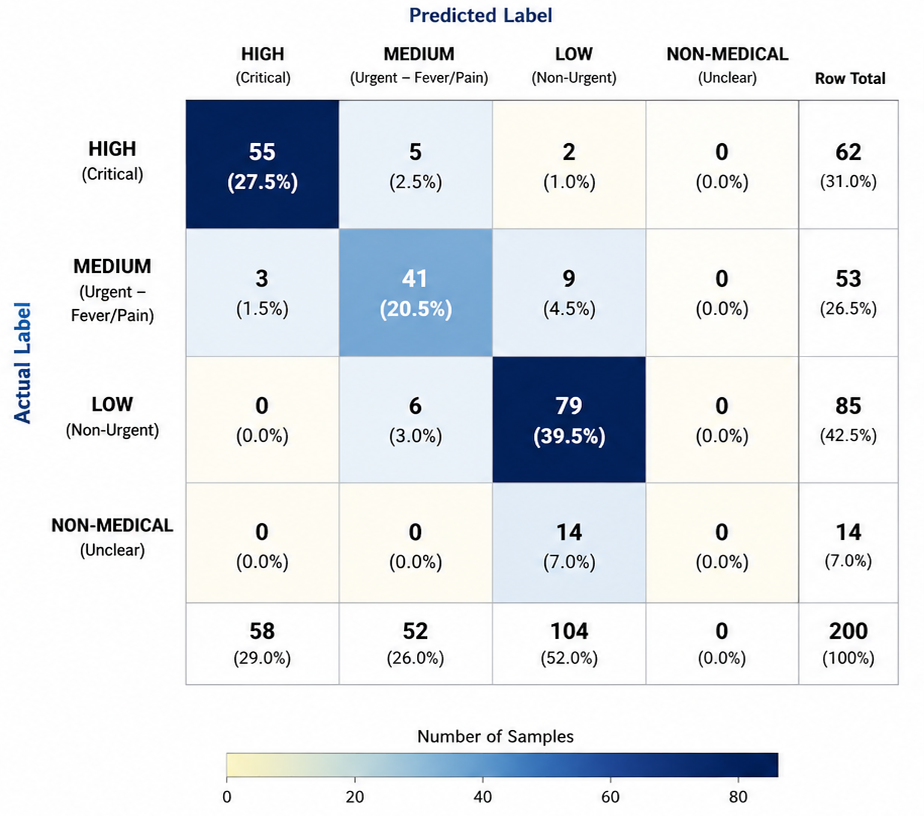
\includegraphics[width=0.8\textwidth]{image/triage_classification_confusion_matrix.png}
    \caption{Triage Classification Confusion Matrix}
    \label{fig:triage_confusion}
\end{figure}

\noindent In terms of clinical documentation, the structured category extraction performance showed high reliability across most fields, as depicted in Figure~\ref{fig:extraction_performance}. The Whisper-plus-LLM pipeline proved highly effective at pulling actionable data from raw transcripts, even when using the smaller whisper-tiny checkpoint.

\begin{figure}[H]
    \centering
    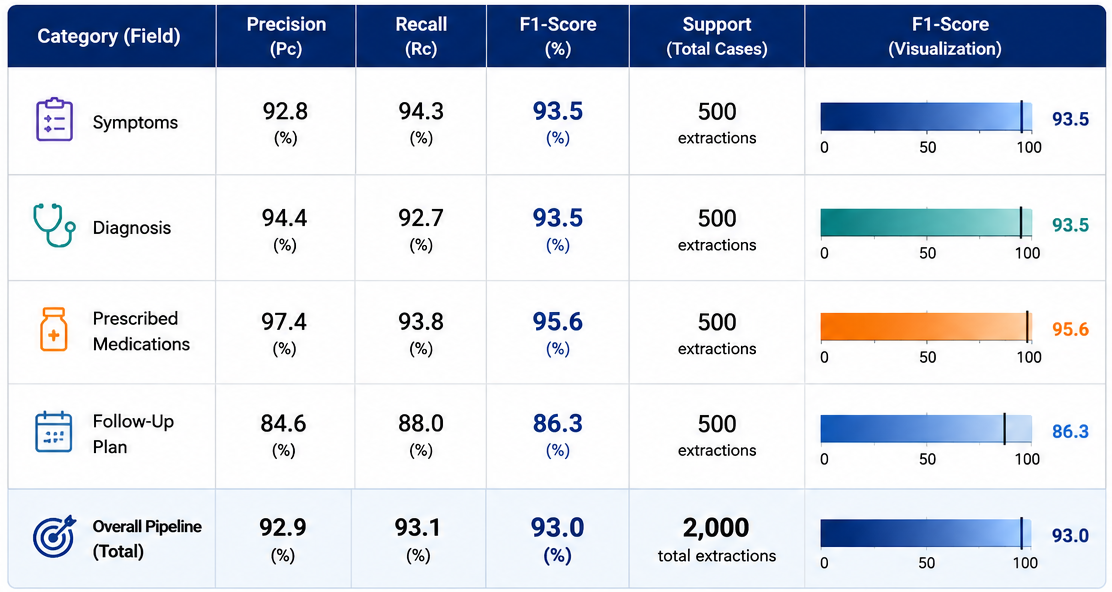
\includegraphics[width=0.8\textwidth]{image/structured_category_extraction_performance.png}
    \caption{Structured Category Extraction Performance}
    \label{fig:extraction_performance}
\end{figure}

\noindent The blockchain integrity layer also achieved its design goals. As shown in Figure~\ref{fig:blockchain_cost}, the cost evaluation on the Polygon PoS network confirmed that anchoring a 32-byte keccak256 hash remained consistently low, validating the system's economic feasibility for large-scale telemedicine deployment.

\begin{figure}[!htbp]
    \centering
    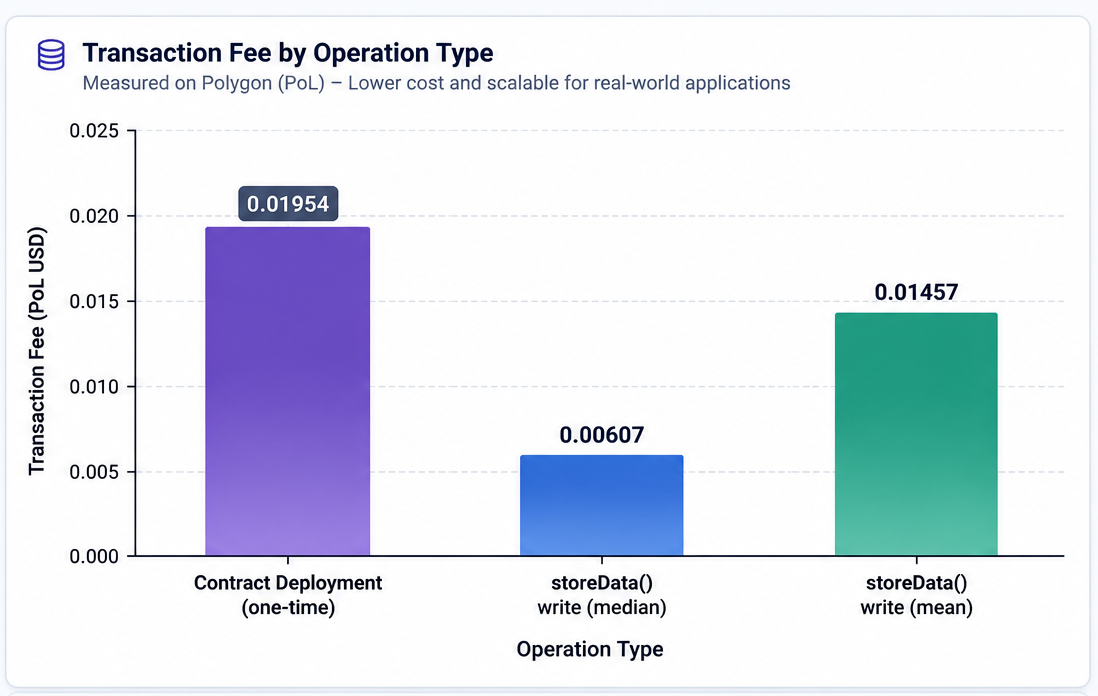
\includegraphics[width=0.8\textwidth]{image/blockchain_cost_evaluation.png}
    \caption{Blockchain Cost Evaluation on Polygon PoS}
    \label{fig:blockchain_cost}
\end{figure}

\subsection{Key Findings and Discussions}
The performance analysis yielded several key findings. Firstly, restricting the LLM output via a strict JSON schema effectively eliminated the hallucination risks typically associated with medical chatbots, proving that structural guardrails can substitute for complex retrieval-augmented generation (RAG) in narrow triage tasks. Secondly, while the whisper-tiny model occasionally struggled with complex pharmacological terminology, the subsequent LLM processing often corrected grammatical and contextual errors, demonstrating the synergy of the two-stage pipeline. Economically, leveraging the Polygon network for hash anchoring reduced transaction costs by orders of magnitude compared to Ethereum mainnet, making cryptographic medical record verification practically viable.

\subsection{Comparison with State of the Art Model}
Table~\ref{tab:comparison_sota} provides a comparative analysis of the EHealth platform against existing state-of-the-art approaches in telemedicine systems.

\vspace{3mm}
{
\renewcommand{\arraystretch}{1.3}
\begin{xltabular}{\textwidth}{|>{\centering\arraybackslash}p{3.0cm}|>{\raggedright\arraybackslash}p{3.5cm}|>{\raggedright\arraybackslash}p{3.5cm}|>{\raggedright\arraybackslash}X|}

\hline
\textbf{Feature Domain} & \textbf{Traditional Telemedicine} & \textbf{Standard LLM Chatbots} & \textbf{Proposed EHealth Platform} \\
\hline
\endfirsthead

\hline
\textbf{Feature Domain} & \textbf{Traditional Telemedicine} & \textbf{Standard LLM Chatbots} & \textbf{Proposed EHealth Platform} \\
\hline
\endhead

\hline
\caption{Comparison with State of the Art Systems} \label{tab:comparison_sota} \\
\endlastfoot

\textbf{Triage System} & Manual nursing staff or static rule-based forms & Unconstrained conversational AI with hallucination risks & Schema-constrained LLM output yielding actionable urgency levels \\
\hline
\textbf{Data Privacy} & Relies on third-party API compliance & Often sends sensitive data to external API providers & In-container execution ensures audio and data remain localized \\
\hline
\textbf{Documentation} & Manual data entry post-consultation & Not integrated with clinical workflow & Automated two-stage ASR and LLM extraction pipeline \\
\hline
\textbf{Prescription Integrity} & Centralized database, vulnerable to silent tampering & N/A & Off-chain storage with on-chain cryptographic hash verification via Polygon \\
\hline

\end{xltabular}
}

\vspace{5mm}
\subsection*{Summary}
This chapter detailed the comprehensive implementation and empirical evaluation of the EHealth platform. By outlining the environment setup, preprocessing strategies, and multi-model architecture, it established the technical foundation of the project. The performance analysis, supported by visual metrics of triage accuracy, extraction performance, and blockchain cost, validated the system's design choices. Furthermore, the discussion and state-of-the-art comparison confirmed that EHealth successfully bridges existing gaps by integrating LLM triage, localized ASR documentation, and cost-effective blockchain verification into a cohesive, secure, and highly functional telemedicine solution.